%%%%%%%%%%%%%%%%%%%%%%%%%%%%%%%%%%%%%%%%%%%%%%%%%%%%%%%%%%%%%%%%%%%%%%%%%%%%%%%%
% Thesis / Project Report
% LaTeX Template
% Version 2.0 (08/04/16)
%
% Author:
% Siddhant Shrivastava
% https://github.com/sidcode/bits-pilani-thesis-template-latex
%
% This template is heavily based on the work of Darshit Shah, Steven Gunn and Sunil Patel
% Darshit Shah
% https://github.com/darnir/BPHC-LaTeX-Report-Class
% Steven Gunn
% http://users.ecs.soton.ac.uk/srg/softwaretools/document/templates/
% and
% Sunil Patel
% http://www.sunilpatel.co.uk/thesis-template/
%
% License:
% CC BY-NC-SA 4.0 (http://creativecommons.org/licenses/by-nc-sa/4.0/)
%
% Note:
% Make sure to edit document variables in the Thesis.cls file
%
%%%%%%%%%%%%%%%%%%%%%%%%%%%%%%%%%%%%%%%%%%%%%%%%%%%%%%%%%%%%%%%%%%%%%%%%%%%%%%%%

%-------------------------------------------------------------------------------
%	PACKAGES AND OTHER DOCUMENT CONFIGURATIONS
%-------------------------------------------------------------------------------

\documentclass[11pt, a4paper, oneside]{Thesis} % Paper size, default font size
                                               % and one-sided paper

\graphicspath{{Pictures/}} % Specifies the directory where pictures are stored

\usepackage[backend=bibtex]{biblatex}
\bibliography{Bibliography.bib}

\usepackage{caption}
\usepackage{subcaption}
\usepackage{algorithm}
\usepackage{algpseudocode}
\usepackage{numprint}
\usepackage{multirow}

\title{\ttitle} % Defines the thesis title - don't touch this


\newcommand{\todo}[1]{\textbf{{\color{red}#1}}\xspace}
\npthousandsep{,}

\begin{document}

\frontmatter % Use roman numbering style (i, ii...) for the pre-content pages

\setstretch{1.3} % Line spacing of 1.3

% Define page headers using FancyHdr package and set up for one-sided printing
\fancyhead{} % Clears all page headers and footers
\rhead{\thepage} % Sets the right side header to show the page number
\lhead{} % Clears the left side page header

\pagestyle{fancy} % Finally, use the "fancy" page style to implement the
                  %FancyHdr headers

% Input all the variables used in the document. Please fill out the
% variables.tex file with all your details.
%-------------------------------------------------------------------------------
%	DOCUMENT VARIABLES
%
%	Fill in the lines below to set the various variables for the document
%-------------------------------------------------------------------------------

%-------------------------------------------------------------------------------
% Your thesis title - this is used in the title and abstract
% Command: \ttitle
% \thesistitle{ P4Campus: Passive Traffic Classification and Monitoring at the edge}
\thesistitle{Understanding TCP Internet Traffic Characteristics through Passive Monitoring at the Campus Edge}
%-------------------------------------------------------------------------------
% The document type: Thesis / report, etc.
% Command: \doctype
\documenttype{Undergraduate Thesis}
%-------------------------------------------------------------------------------
% Your supervisor's name - this is used in the title page
% Command: \supname
\supervisor{Dr. Ben \textsc{Leong}}
%-------------------------------------------------------------------------------
% The supervisor's position - Used on Certificate
% Command: \suppos
\supervisorposition{Associate Professor}
%-------------------------------------------------------------------------------
% Supervisor's institute
% Command: \supinst
\supervisorinstitute{National University of Singapore}
%-------------------------------------------------------------------------------
% Your Co-Supervisor's name
% Command: \cosupname
\cosupervisor{Dr. Virendra Singh \textsc{Shekhawat}}
%-------------------------------------------------------------------------------
% Co-Supervisor's Position - Used on Certificate
% Command: \cosuppos
\cosupervisorposition{Associate Professor}
%-------------------------------------------------------------------------------
% Co-Supervisor's Institute
% Command: \cosupinst
\cosupervisorinstitute{BITS-Pilani Pilani Campus}
%-------------------------------------------------------------------------------
% Your Examiner's name. Not currently used anywhere.
% Command: \examname
\examiner{}
%-------------------------------------------------------------------------------
% Name of your degree
% Command: \degreename
\degree{Bachelor of Engineering (Hons.) Computer Science}
%-------------------------------------------------------------------------------
% The BITS Course Code for which this report is written
% COmmand: \ccode
\coursecode{BITS F422T}
%-------------------------------------------------------------------------------
% The name of the Course
% Command: \cname
\coursename{Thesis}
%-------------------------------------------------------------------------------
% Your name. Extend manually in case of multiple authors
% Command: \authornames
\authors{Satvik \textsc{Sinha}}
%-------------------------------------------------------------------------------
% Your ID Number - used on the Title page and abstract
% Command: \idnum
\IDNumber{2020A7TS0993P}
%-------------------------------------------------------------------------------
% Your address
% Command: \addressnames
\addresses{}
%-------------------------------------------------------------------------------
% Your subject area
% Command: \subjectname
\subject{}
%-------------------------------------------------------------------------------
% Keywords for this report.
% Command: \keywordnames
\keywords{}
%-------------------------------------------------------------------------------
% University details
% Command: \univname
\university{\texorpdfstring{\href{http://www.bits-pilani.ac.in/} % URL
                {Birla Institute of Technology and Science Pilani, Pilani Campus}} % University name
                {Birla Institute of Technology and Science Pilani, Pilani Campus}}
%-------------------------------------------------------------------------------
% University details, in Capitals
% Command: \UNIVNAME
\UNIVERSITY{\texorpdfstring{\href{http://www.bits-pilani.ac.in/} % URL
                {BIRLA INSTITUTE OF TECHNOLOGY AND SCIENCE PILANI, PILANI CAMPUS}} % name in capitals
                {BIRLA INSTITUTE OF TECHNOLOGY AND SCIENCE PILANI, PILANI CAMPUS}}
%-------------------------------------------------------------------------------
% Department Details
% Command: \deptname
\department{\texorpdfstring{\href{http://www.bits-pilani.ac.in/pilani/computerscience/ComputerScience} % Your department's URL
                {Computer Science \& Information Systems}} % Your department's name
                {Computer Science}}
%-------------------------------------------------------------------------------
% Department details, in Capitals
% Command: \DEPTNAME
\DEPARTMENT{\texorpdfstring{\href{http://www.bits-pilani.ac.in/pilani/computerscience/ComputerScience} % Your department's URL
                {COMPUTER SCIENCE \& INFORMATION SYSTEMS}} % Your department's name in capitals
                {COMPUTER SCIENCE \& INFORMATION SYSTEMS}}
%-------------------------------------------------------------------------------
% Research Group Details
% Command: \groupname
\group{\texorpdfstring{\href{Research Group Web Site URL Here (include http://)}
                {Research Group Name}} % Your research group's name
                {Research Group Name}}
%-------------------------------------------------------------------------------
% Research Group Details, in Capitals
% Command: \GROUPNAME
\GROUP{\texorpdfstring{\href{Research Group Web Site URL Here (include http://)}
                {RESEARCH GROUP NAME (IN BLOCK CAPITALS)}}
                {RESEARCH GROUP NAME (IN BLOCK CAPITALS)}}
%-------------------------------------------------------------------------------
% Faculty details
% Command: \facname
\faculty{\texorpdfstring{\href{Faculty Web Site URL Here (include http://)}
                {Faculty Name}}
                {Faculty Name}}
%-------------------------------------------------------------------------------
% Faculty details, in Capitals
% Command: \FACNAME
\FACULTY{\texorpdfstring{\href{Faculty Web Site URL Here (include http://)}
                {FACULTY NAME (IN BLOCK CAPITALS)}}
                {FACULTY NAME (IN BLOCK CAPITALS)}}
%-------------------------------------------------------------------------------


%-------------------------------------------------------------------------------
%   NON-CONTENT PAGES
%-------------------------------------------------------------------------------
\maketitle
\Declaration
\Certificate
% \Quotation{Insert Random Quote here. Publish like a boss.}{Your Name}

\begin{abstract}
Congestion Control Algorithms (CCAs) play an important role in allowing multiple flows to share the available bandwidth in a network in an equitable way and generally maintain the stability of the internet. In the past, the Internet's stability was guaranteed by the homogeneity of the deployed CCAs. These algorithms have generally been predictable and well-behaved. However. this is quickly changing with the deployment of QUIC, BBR, and numerous other industry-led transport technologies. We now find new transport stacks and CCAs being deployed without much scrutiny. Under this new operating environment, it is crucial to study the deployment of these algorithms at the edge and how they impact the network and other flows that share the same bottleneck. In this thesis, we describe the design and deployment of a new passive measurement testbed called {\em CampusMeasure}.
\end{abstract}

\begin{acknowledgements}
I would like to thank my supervisor, Dr. Ben \textsc{Leong} for providing me an opportunity to work with his research group at the National University of Singapore. I am also grateful to my mentors, Raj Joshi, Ayush Mishra and Archit Bhatnagar for helping me throughout in any problems I faced. I would also like to thank Dr. Virendra Singh \textsc{Shekhawat} for his support and guidance during the weekly meetings of the research group. Lastly I would like to thank my family and friends for their constant support and motivation.
\end{acknowledgements}

%-------------------------------------------------------------------------------
%	LIST OF CONTENTS/FIGURES/TABLES PAGES
%-------------------------------------------------------------------------------

% The page style headers have been "empty" all this time, now use the "fancy"
% headers as defined before to bring them back
\pagestyle{fancy}

\lhead{\emph{Contents}} % Set the left side page header to "Contents"
\tableofcontents % Write out the Table of Contents

% Set the left side page header to "List of Figures"
\lhead{\emph{List of Figures}}
\listoffigures % Write out the List of Figures

%  % Set the left side page header to "List of Tables"
% \lhead{\emph{List of Tables}}
% \listoftables % Write out the List of Tables

%-------------------------------------------------------------------------------
%	ABBREVIATIONS
%-------------------------------------------------------------------------------

\clearpage % Start a new page

 % Set the line spacing to 1.5, this makes the following tables easier to read
\setstretch{1.5}

\lhead{\emph{Abbreviations}} % Set the left side page header to "Abbreviations"
\listofsymbols{ll} % Include a list of Abbreviations (a table of two columns)
{
% \textbf{LAH} & \textbf{L}ist \textbf{A}bbreviations \textbf{H}ere \\
%\textbf{Acronym} & \textbf{W}hat (it) \textbf{S}tands \textbf{F}or \\
\textbf{RTT} & \textbf{R}ound \textbf{T}rip \textbf{T}ime \\
\textbf{BBR} & \textbf{B}ottleneck \textbf{B}andwidth and \textbf{R}ound-trip propagation time \\
\textbf{IP} & \textbf{I}nternet \textbf{P}rotocol  \\
\textbf{TCP} & \textbf{T}ransmission \textbf{C}ontrol \textbf{P}rotocol \\
\textbf{UDP} & \textbf{U}ser \textbf{D}atagram \textbf{P}rotocol \\
\textbf{QUIC} & \textbf{Q}uick \textbf{U}DP \textbf{I}internet \textbf{C}onnections \\
\textbf{CCA} & \textbf{C}ongestion \textbf{C}control \textbf{A}lgorithm \\
\textbf{DPDK} & \textbf{D}ata \textbf{P}lane \textbf{D}evelopment \textbf{K}it \\
}

%-------------------------------------------------------------------------------
%	PHYSICAL CONSTANTS/OTHER DEFINITIONS
%-------------------------------------------------------------------------------

% \clearpage % Start a new page

% Set the left side page header to "Physical Constants"
% \lhead{\emph{Physical Constants}}

 % Include a list of Physical Constants (a four column table)
% \listofconstants{lrcl}
% {
% Speed of Light & $c$ & $=$ & $2.997\ 924\ 58\times10^{8}\ \mbox{ms}^{-\mbox{s}}$ (exact)\\
% Constant Name & Symbol & = & Constant Value (with units) \\
% }

%-------------------------------------------------------------------------------
%	SYMBOLS
%-------------------------------------------------------------------------------

% \clearpage % Start a new page

% \lhead{\emph{Glossary}} % Set the left side page header to "Symbols"

% \listofnomenclature % List the nomenclature. (We use the glossaries package)

%-------------------------------------------------------------------------------
%	DEDICATION
%-------------------------------------------------------------------------------

\setstretch{1.3} % Return the line spacing back to 1.3

\pagestyle{empty} % Page style needs to be empty for this page

% Dedication text
% \Dedicatory{Dedicate this to someone, anyone.}

\addtocontents{toc}{\vspace{2em}} % Add a gap in the Contents, for aesthetics

%-------------------------------------------------------------------------------
%	THESIS CONTENT - CHAPTERS
%-------------------------------------------------------------------------------

\mainmatter % Begin numeric (1,2,3...) page numbering

\pagestyle{fancy} % Return the page headers back to the "fancy" style

% Include the chapters of the thesis as separate files from the Chapters folder
% Uncomment the lines as you write the chapters

% Chapter 1

\chapter{Introduction} % Main chapter title

\label{Chapter1} % For referencing the chapter elsewhere, use \ref{Chapter1} 

\lhead{Chapter 1. \emph{Introduction}} % This is for the header on each page - perhaps a shortened title

%----------------------------------------------------------------------------------------
% Why are we doing these measurements?
The Internet supports many applications like IoT devices, live video streaming, and online stock trading, with different requirements. The infrastructure and the technologies supporting the internet have advanced, bringing link speeds to hundreds of gigabits per second and packet processing delays to the order of nanoseconds on the latest switching hardware. The evolving landscape has seen increased video traffic~\cite{gipr-sandvine22} and other low-latency-requiring applications. New technologies have been developed and deployed on the internet to cater to the new needs. Google has developed BBR~\cite{bbrgoogle-acmqueue16}, a new CCA to perform better in lossy networks and provide low latencies. Similarly, QUIC~\cite{quic-sigcomm17} is a new user-space transport stack that gives users more flexibility to deploy new CCAs. Recent developments have led to a rapidly evolving congestion control landscape and a need to monitor these new algorithms at the edge to study their impact on the network.

Designing new algorithms for the network for tasks like congestion control and active queue management requires us to be aware of many network hyper-parameters like flow size, flow duration, number of concurrent flows and RTT distribution amongst others. Our best estimates of these metrics are quite outdated~\cite{tcprtt-imc03,revisittcp-imc21,2004-shakkottai-t20}, and their measurements must be replenished in correspondence to the changing Internet landscape. The campus of NUS serves as a unique vantage point in the measurement of these key metrics. Since in most cases, the bottleneck lies near the client (edge of the network), these measurements will be helpful in the development of future congestion control algorithms.
The measurements will also help diagnose potential network issues like microbursts/heavy hitters, buffer overflows, and increases in latencies. It aids in facilitating the network operator to have fine-grained network metrics to resolve various other problems associated with the campus network. 

% What are we doing?
In this thesis, we describe the design and implementation of a testbed that will allow us to measure several important parameters of flows that are part of the traffic going through the campus' gateway router. We use these measurement to detect congestion events by measuring link utilization, packet losses and the RTT values of the flows part of the congested links.

% How are we doing?
\section{Experimental Setup}

We deploy our passive measurement testbed to study and monitor live internet traffic at the edge of our campus network. The vantage point that meets this criterion and offers maximum insight into the network would be the links connecting the gateway router of the campus network.

\begin{figure}[t]
    \centering
        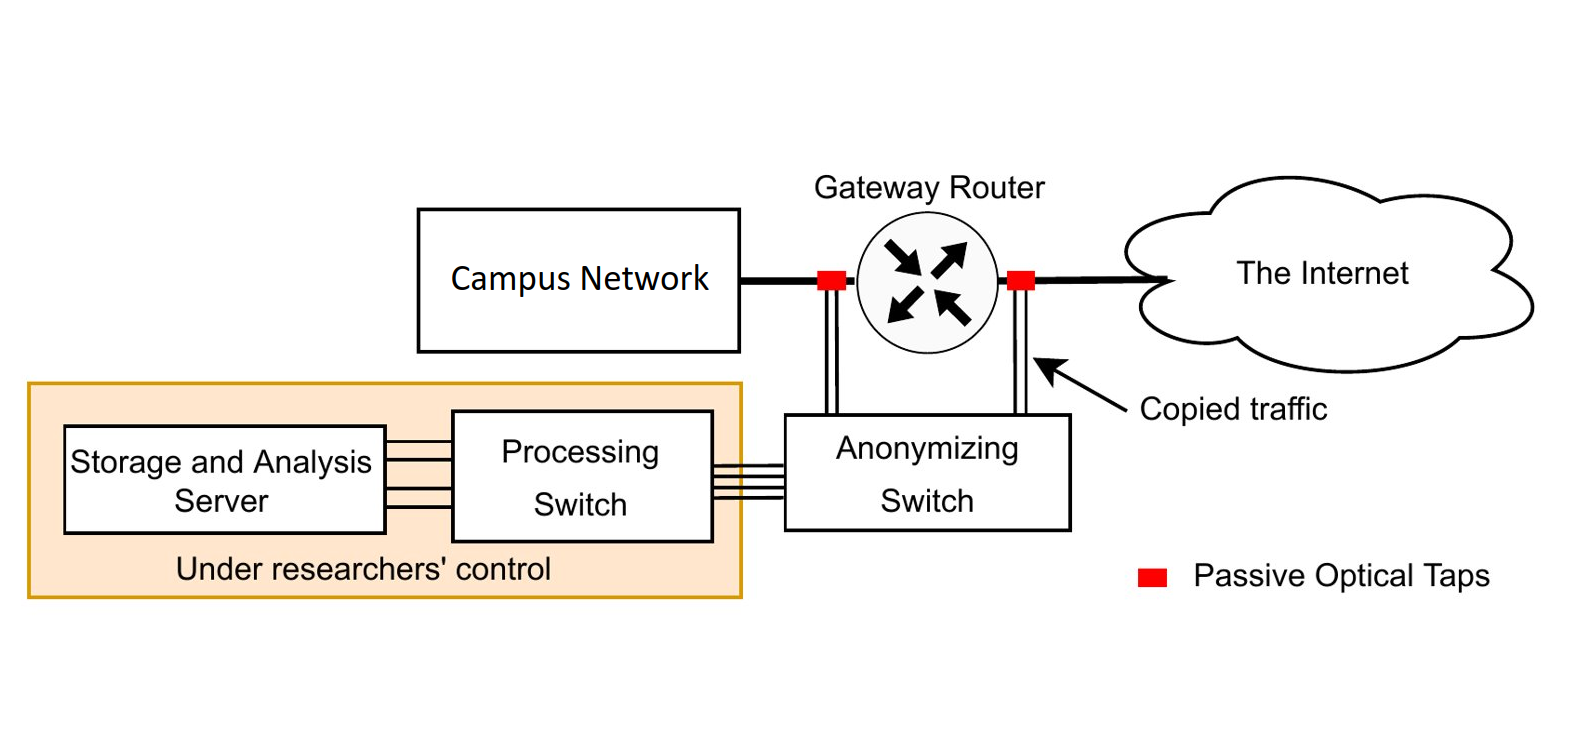
\includegraphics[width=\textwidth]{Figures/setup.png}
    \caption[Experimental Setup]{Experimental Setup}
    \label{fig:setup}
    \bigskip
\end{figure}

Figure \ref{fig:setup} shows how we tap live traffic from the network links connecting our campus to the internet. The gateway router is connected to the campus network using 10G optical links. We tap the links using a passive optical tap to obtain a copy of the traffic at the line rate. The device splits the optical signal into two identical copies without affecting the rate of the traffic. The mirrored traffic is passed across to the anonymizing switch. The anonymizing switch has been used to ensure the privacy of the users and is under the control of the network operators. The anonymizing switch anonymizes the packet by encrypting the source and destination IP addresses and TCP ports by a custom anonymization mechanism. It also truncates the TCP/UDP payload. After doing this, it adds a custom header in between the Ethernet and IP headers of the packet to preserve some telemetry information of the packet such as packet length, packet timestamp, and header length. It then forwards the anonymized packets to the processing switch. The processing switch then passes the uplink and downlink traffic to different ports on the storage analysis server to do different computations on the traffic.

\section{Packet Structure}

\begin{figure}[t]
    \centering
        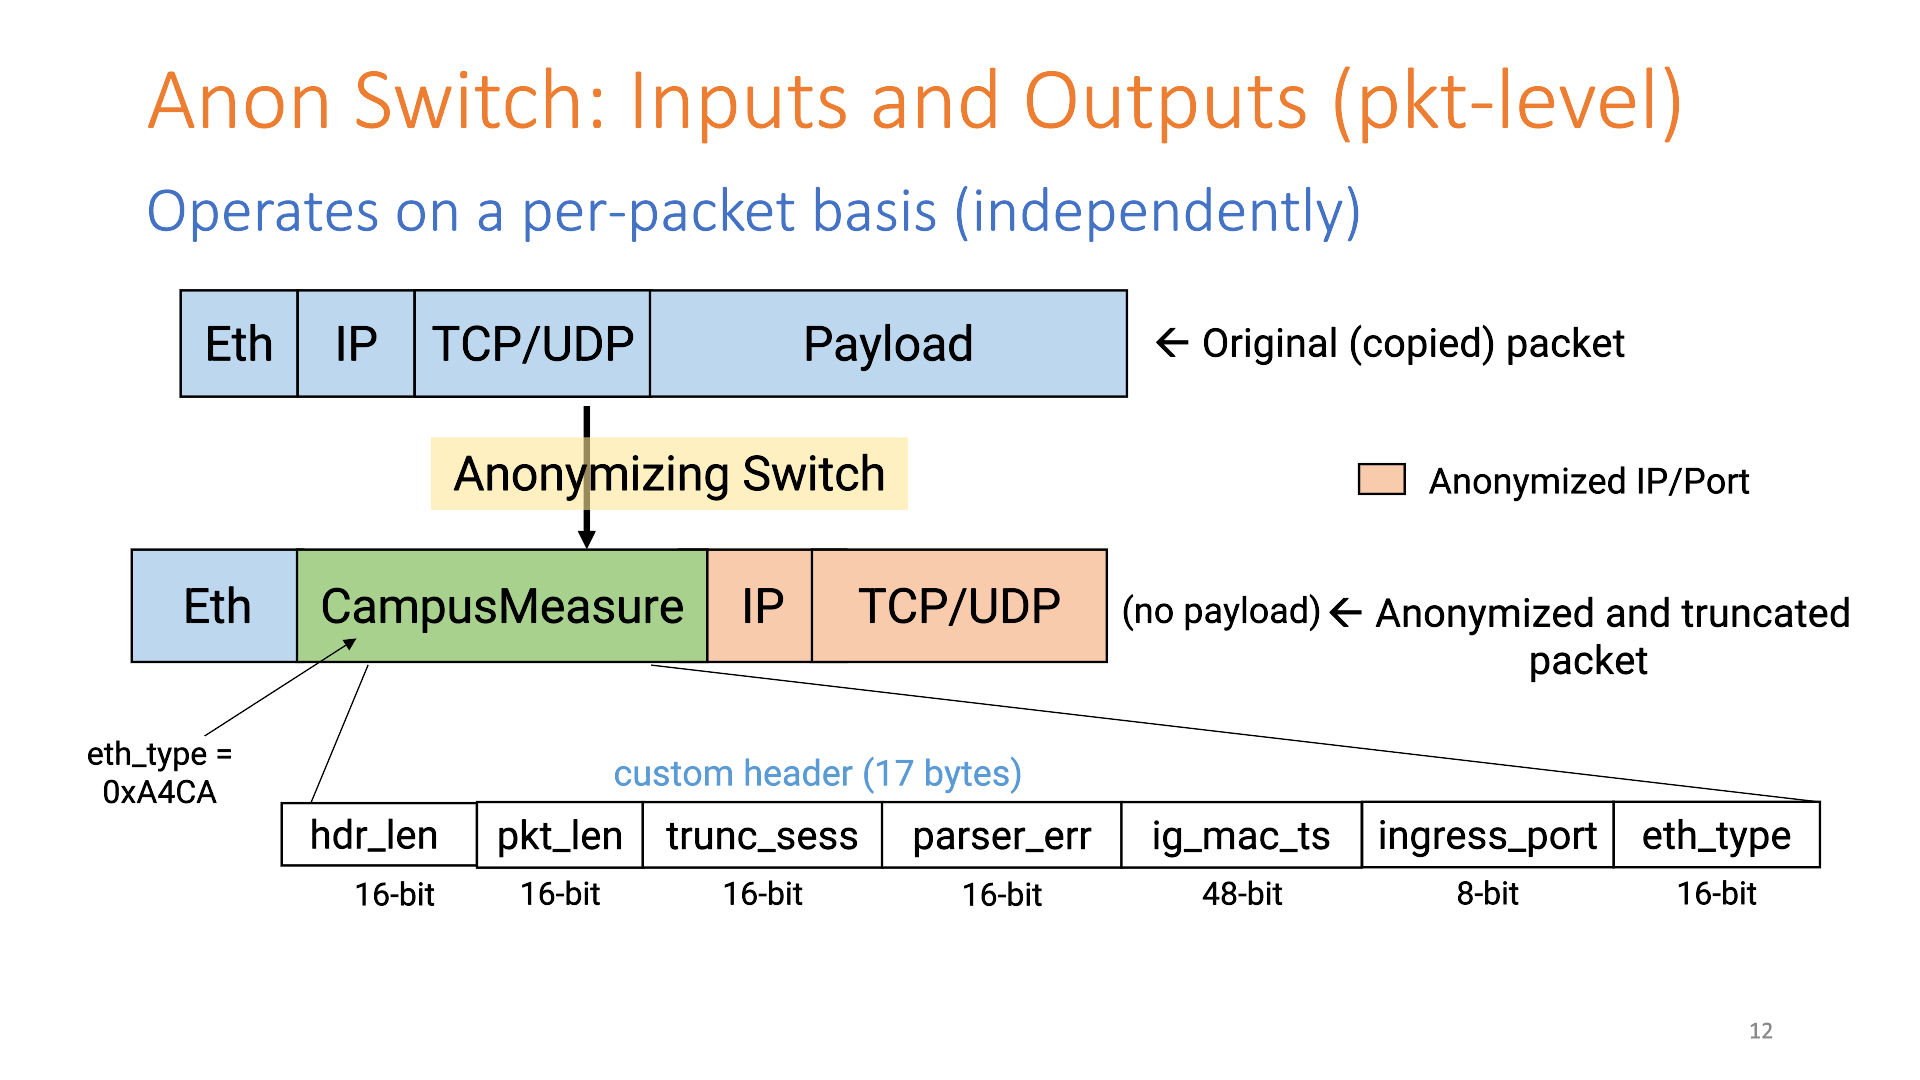
\includegraphics[width=\textwidth]{Figures/pkt-struct.png}
    \caption[Packet structure]{Packet structure}
    \label{fig:struct}
    \bigskip
\end{figure}

Figure \ref{fig:struct} shows the structure of the packet after anonymization by the switch. It inserts a new header field of 17 bytes called the CampusMeasure Header in between the Ethernet and the IP fields.
The most important fields in this new header are the $hdr\_len,pkt\_len$ and $ig\_mac\_ts$ fields. The ingress mac time-stamp is recorded as the packet is received at the ingress port of the switch. The packet length is the total length of the packet before the truncation. These two fields are used to do most of our computations in the later sections such as calculating the link utilization, flow duration etc.

\section{Packet capture at the server}

Traditional packet capture tools such as tcpdump~\cite{tcpdump} operate in the kernel space of the operating system. The functioning of these tools involve context switching between the user and kernel space which adds additional overhead. This overhead causes latency and can lead to packet drops in an environment involving high packet rates. These tools also generally use inefficient memory management techniques compromising system performance.

\begin{figure}[t]
    \centering
        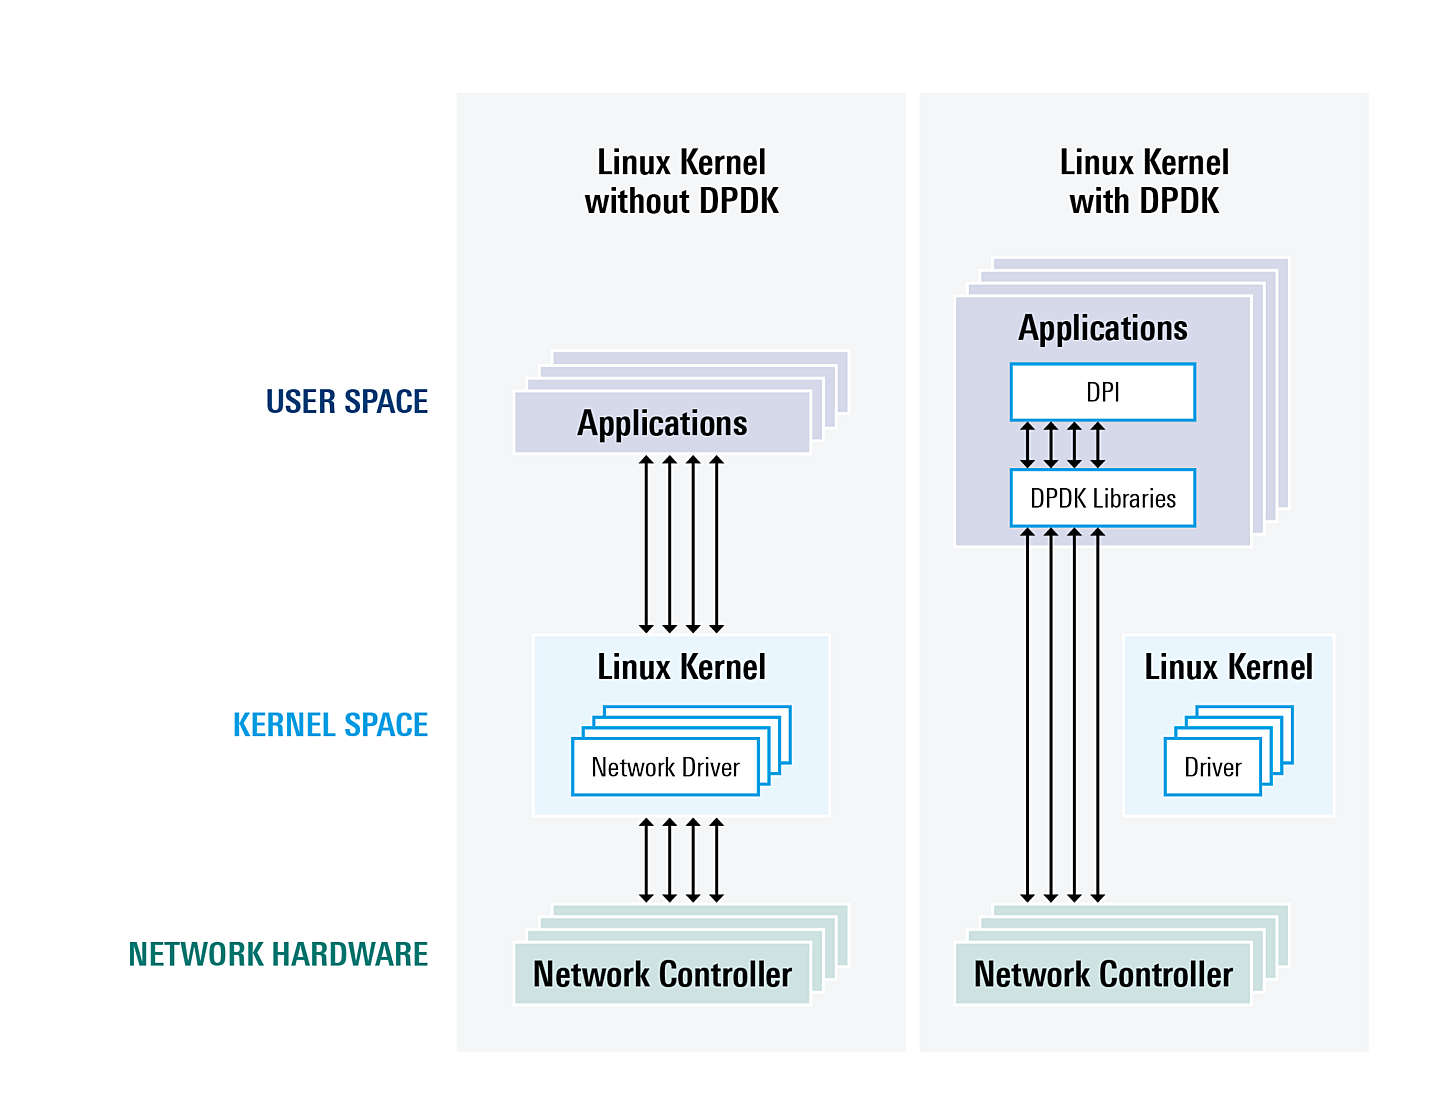
\includegraphics[width=\textwidth]{Figures/dpdk.png}
    \caption[DPDK Approach]{DPDK Approach ~\cite{dpdk2023}}
    \label{fig:dpdk}
    \bigskip
\end{figure}

Instead of these traditional tools, we use DPDK~\cite{dpdk} to capture packets at high rates efficiently. As shown in Figure \ref{fig:dpdk}, DPDK bypasses the operating system kernel and directly accesses network hardware. As a result of bypassing the kernel space, and handling packet processing in the user space itself, DPDK achieves lower latency and can capture packets without any drops even at rates such as 10 Gbps. We write a packet capture program in C using DPDK libraries to capture traffic from the two ports of the server simultaneously using two worker threads and write the captured packets to two separate pcap files.

We then modify the tool to customize packet captures. We can input the duration of packet capture, the frequency after which to start the next capture, and the start and end times of the packet capture, and the packet capture would run to create separate pcap files(uplink and downlink) for each capture.
%----------------------------------------------------------------------------------------
% Chapter Template

\chapter{Related Work} % Main chapter title

\label{Chapter2} % Change X to a consecutive number; for referencing this chapter elsewhere, use \ref{ChapterX}

\lhead{Chapter 2. \emph{Related Work}} % Change X to a consecutive number; this is for the header on each page - perhaps a shortened title

%----------------------------------------------------------------------------------------

% Several attempts have been made in the past to measure the internet traffic.

In this section, we'll review the work done on internet measurement. It has been further subdivided into two sections. The first section talks about the measurements done using P4 programmable switches by the P4Campus group at Princeton. The second section talks about other internet measurements done to better our understanding of transport protocols.

\section{P4Campus at Princeton}

\begin{figure}[t]
    \centering
        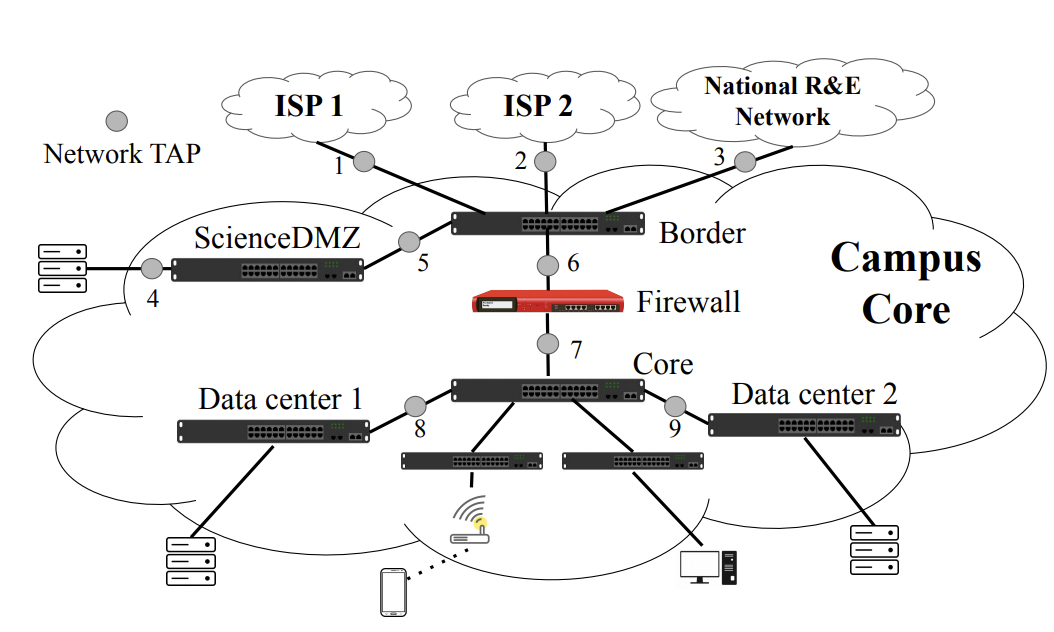
\includegraphics[width=\textwidth]{Figures/image.png}
    \caption[P4Campus]{P4Campus ~\cite{p4campusprinceton}}
    \label{fig:p4camp}
    \bigskip
\end{figure}

The P4Campus project~\cite{p4campusprinceton} at Princeton University is very similar to our CampusMeasure project in terms of the setup used. The backbone of their setup is the same as ours. Figure \ref{fig:p4camp} shows the key differences between the two setups. They have tapped the links at multiple points, whereas we tap the links at only one point(at the gateway router). They use a custom anonymization policy ONTAS~\cite{ontas-netai19} which performs line rate anonymization of traffic, with the option of encrypting ethernet and IP headers on programmable switches using P4. They also don't perform payload truncation contrary to our policy.

Their group has made several measurements over the years with the help of their setup in their campus network. The group focuses on implementing systems in the data plane using the P4~\cite{p4lang} language to make measurements. Dart~\cite{dart-sigcomm22} is a system that performs continuous in-network RTT estimation in the data plane by passively measuring internet traffic. The system maintains a packet-tracker table, by creating an entry in a hash table using the four-tuple of the flow and the expected ACK number as the key, and the timestamp as the value. It then matches the corresponding ACK packet and measures the RTT by calculating the difference in the two timestamps. The system also avoids ambiguous RTT measurements caused due to packet losses and re-ordering, by maintaining a range tracker table for each flow. The range tracker maintains a valid range of sequence numbers for a flow and collapses the range in case of a packet loss or re-transmission event. Oliver et al.~\cite{zoom-imc22} perform passive measurements on Zoom's custom RTP header to measure fine-grained metrics like media-bit rates, delay-frame rates, frame-level jitter, and retransmission. They perform an entropy-based packet header analysis for an RTP packet by plotting the header values on a graph for different packets, in order to decipher different fields of the unknown packet. Sherry et al.~\cite{osfingerprint-netsoft22} performed experiments to fingerprint operating systems on commodity switches passively to detect OS-specific vulnerabilities and administer OS-related security policies that block, rate-limit, or redirect traffic. They determine OS-specific fingerprints based on the TCP and IP header values of a packet. Upon encountering a packet, they match the TCP and IP header values with the existing signatures to determine the OS. The TCP options are used for more specific fingerprinting. Jason et al.~\cite{domainnameanalysis-sosr21} characterize traffic using high-level indicators like domain name instead of IP address in the data plane. They extract the domain names queried by clients by tracking the DNS response packets along with the client and server IP addresses and store them in a hash table. They then keep track of the count of the data packets from the server to the client to measure the traffic volume per flow. Chen et al.~\cite{conquest-conext19} perform fine-grained queue measurement to identify flows contributing to queue(FIFO) buildup and latency. The routers are tapped on both ends to determine the arrival and departure times of the packets. They measure the queuing delay for a packet by capturing the arrival and departure times, and if the delay is greater than a certain threshold, they check for flows contributing to the queue buildup. The percentage of packets of each flow in the queue is calculated and flows contributing to queue buildup are reported. Ben-Basat et al.~\cite{probabilisticrecirculation-icnp2018} find heavy hitter flows in the queues by using counter-based algorithms. They maintain a hash table to count the number of packets per flow and increment the counter each time a packet of the flow arrives. If the flow is not already present in the hash table, they probabilistically re-circulate the packet to avoid processing delay each time, per the high switch speed. If in case the table is full, the flow with the minimum count is evicted.

\section{Other Internet measurement techniques}

RTT measurements on the internet traffic have been made since a long time. Some of the most fundamental tools like ping~\cite{iputils} and traceroute~\cite{inetutils} use active measurement techniques to measure RTT for a flow. Active measurement techniques may not always produce accurate results as they might increase congestion in an already congested network. Studies have shown that the RTT measurements made by ping are not very accurate because of flow-level load balancing done by network routers, resulting in different traffic routes for ICMP ping packets ~\cite{paris2tokyoping-imc13}. Passive measurement of RTT done by analysing the TCP handshake might not be enough as shown by Jay et al.~\cite{tcprtt-imc03}. They recorded one of the first RTT measurements passively between endpoints at a large university campus.Their studies showed that the RTT values vary widely over a time for a long flow. Shakkottai et al. ~\cite{2004-shakkottai-t20} measured the RTT distribution of TCP flows using different methods and its impact on TCP-based flow control.

Feng et al. ~\cite{tcprevisited-imc09} determine the initial congestion window size, irregular retransmission events and TCP flow clocking by analyzing uni-directional TCP flows. They calculate the ICW size using an algorithm that identifies the first large gap between the sending of two packets by the server. They also detect irregular retransmissions by the sender. by statistically checking if there is a negative correlation between the retransmission rate and the sending rate. They extract the TCP flow clock from the uni-directional trace using Fourier transforms.  Raman et al.~\cite{tampering-sigcomm23} detect connection tampering done by middleboxes by passively comparing TCP flows with certain tampering signatures. The tampering signatures are a comprehensive list of sequences of TCP header packets that are indicative of a tampering event. Some of the frequent signatures observed by them were tampering mid-TCP handshake and immediately after the TCP handshake. Debopam et al.~\cite{latency-imc20} reconstructed licensed financial trading networks to examine their latency, wireless link lengths, path redundancy, and other features. Benko et al.~\cite{1189102} calculate packet losses passively by using the TCP sequence numbers and noticing the retransmissions and re-ordering events. They refine their measurements by calculating loss rates only for significant packets and ignoring the packets for which the loss is too uncertain like the first and last data segments of a flow and re-transmitted packets. Joel et al.~\cite{10.1145/1090191.1080111}
tried improving the accuracy in end-to-end packet loss measurement using active probes by Zing~\cite{707817}, a tool that sends UDP packets at Poisson-modulated intervals with a fixed mean rate.
%----------------------------------------------------------------------------------------
% Chapter Template

\chapter{Methodology} % Main chapter title

\label{Chapter3} % Change X to a consecutive number; for referencing this chapter elsewhere, use \ref{ChapterX}

\lhead{Chapter 3. \emph{Methodology}} % Change X to a consecutive number; this is for the header on each page - perhaps a shortened title

%----------------------------------------------------------------------------------------

% \section{Testing the Demo Setup before Actual Deployment}

% We created a demo setup to test a few things before the actual deployment of the hardware. For that purpose, we created two namespaces on our server, one for denoting the Internet, and the other for denoting SoC (NUS Campus) as shown in figure \ref{fig:demo}. 

% \begin{figure}[h]
%     \centering
%         \includegraphics[width=\textwidth]{Figures/demo_setup.png}
%     \caption[Demo Setup]{DDemo Setup}
%     \label{fig:demo}
%     \bigskip
% \end{figure}

% We then wrote a client program in Python that can spawn multiple clients to generate different amounts of load on the bottleneck link and plotted a graph of the number of clients vs the load on the bottleneck link to get an idea of the number of clients needed to reach different throughput rates. We also tested the anonymization of our packets to ensure that the TCP/UDP payload was truncated and the IP addresses and TCP ports were anonymized.

We took measurements of key metrics in the network by designing suitable algorithms for each one of them. The scripts were written in C++ using the PcapPlusPlus~\cite{pcapplusplus} library to ensure fast computation involving large pcap files(in the order of gigabytes).

\section{Link Utilization}

\begin{figure}[t]
    \centering
        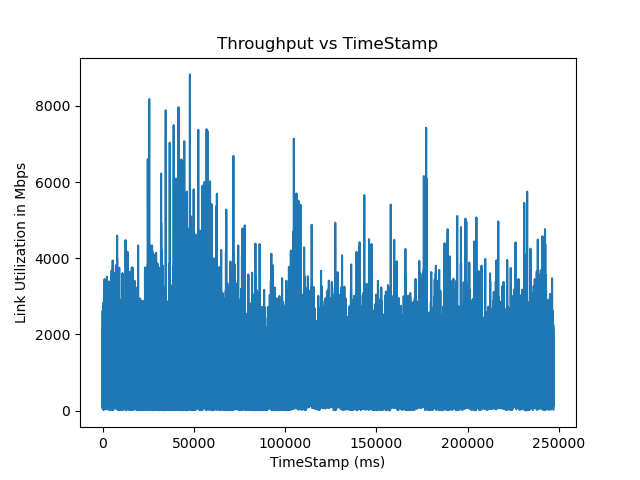
\includegraphics[width=0.75\textwidth]{Figures/link_util_600us.png}
    \caption[Link utilization for a trace]{Link utilization for a trace}
    \label{fig:linkutil}
    \bigskip
\end{figure}

Link utilization is a key metric in detecting congestion events in the network. If the bottleneck link becomes saturated, it can lead to congestion in the link. Link utilization can be computed in two ways. One method involves calculating the throughput for each packet i.e. \( n_b / (t_c - t_p) \) where \(n_b\) is the number of bytes in the packet and \(t_p\) and \(t_c\) are the timestamps of the previous and current packet respectively. Calculating the link utilization at the packet level can take a lot of time. We use a window and stride-based approach for calculating the link utilization. The throughput is calculated as \( \Sigma n_b / (t_w - t_1) \), where \( \Sigma n_b \) represents the sum of the number of bytes sent in the specified time window $w$ and, \(t_1\) and \(t_w\) represent the timestamp of the first and the last packet in the window respectively. The window is then moved by a stride $s$ (time-duration) and the process is repeated for the packets falling in the window. Figure \ref{fig:linkutil} shows the graph for Link Utilization (in Mbps) vs the Timestamp (in ms) for one of the traces captured at our server.

\begin{figure}[t]
    \centering
        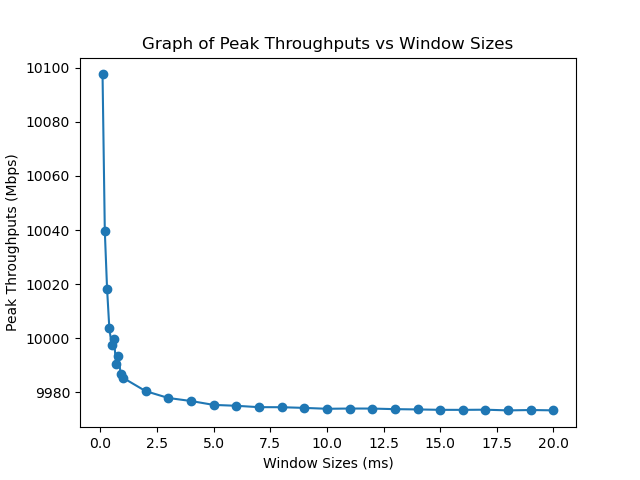
\includegraphics[width=0.75\textwidth]{Figures/peak_vs_window.png}
    \caption[Peak throughput vs window size]{Peak throughput vs window size}
    \label{fig:peak}
    \bigskip
\end{figure}

One of the key challenges while calculating link utilization is to calculate the appropriate window and stride sizes. The approach we used for calculating the suitable window size involved plotting a graph of peak throughput vs the window size in ms. If the window size is too small, it might even be less than the time it takes for a packet to serialize on the link and we will get very large throughput values. If the window size is too large, the peaks will get averaged out and we will get lower throughput values. Thus, the correct estimation of window size is necessary. Figure \ref{fig:peak} shows the optimal window size to be around 0.4 ms, as it is the first point at which the peak throughput is less than the link capacity ($10 Gbps$), and the time window is greater than the time it takes for a packet to serialize. Also, this is the point at which the slope of the graph decreases drastically. The time window is also not large enough to average out peak throughputs. We choose the stride size as half the window size for simplicity.
%----------------------------------------------------------------------------------------

\section{RTT}

RTT calculation is another key metric that also helps in congestion detection. The increase in the RTT of a flow can be attributed to a congestion event. Algorithm \ref{alg:rtt} showcases the approach we use to calculate RTT for different flows throughout their lifetime, which is inspired by Dart~\cite{dart-sigcomm22}.

\begin{algorithm}[ttpb]
\bigskip
\begin{algorithmic}
\State initialize $packettracker$,$rangetracker$ \Comment{intitialization of the two hash tables}
\State read $packet_d$ from $downlink$
\State read $packet_u$ from $uplink$
\While{$downlink$ and $uplink$}
\If{\(packet_d.ts < packet_u.ts\)}
    \If{\(expectedack > rangetracker[flow].right\)}
        \State $rangetracker[flow].right \gets expectedack$
        \State $packettracker[flow] \gets packet_d.ts$
    \Else 
        \State $rangetracker[flow].left \gets rangetracker[flow].right$
    \EndIf
    \State read $packet_d$ from $downlink$
\Else
    \If{$ack$ between $rangetracker[flow].left$ and $rangetracker[flow].right$}
        \State $rangetracker[flow].left \gets ack$
        \State $RTT \gets packet_u$ - $packettracker[flow]$
    \ElsIf{$ack$ == $rangetracker[flow].left$}
        \State  $rangetracker[flow].left \gets rangetracker[flow].right$
    \EndIf
    \State read $packet_u$ from $uplink$
\EndIf
\EndWhile
\end{algorithmic}
\caption[RTT calculation]{RTT calculation}
\label{alg:rtt}
\bigskip
\end{algorithm}

\begin{figure}[t]
    \centering
        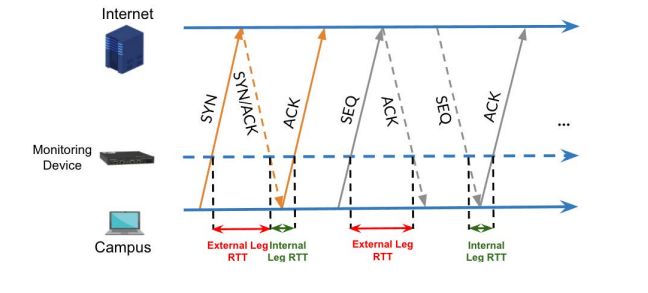
\includegraphics[width=0.8\textwidth]{Figures/rtt.png}
    \caption[RTTs of different legs]{RTTs of different legs ~\cite{dart-sigcomm22}}
    \label{fig:rtt}
    \bigskip
\end{figure}

The algorithm maintains two hash tables: the $packettracker$ table and the $rangetracker$ table for a flow. The $packetracker$ table stores the timestamps for the data packets belonging to a flow and matches the corresponding ACK packets to calculate and store the $RTT$. The $rangetracker$ table ensures that there are no ambiguous $RTT$ measurements. It maintains a range of valid sequence numbers for a flow, where the left edge represents the last ACKed byte by the receiver, and the right edge represents the last byte sent by the sender. The left edge moves when a new packet is ACKed, and the right edge moves when a new packet is sent. If the sequence number of data packet is less than the right edge or if the acknowledgment number of an ACK packet is equal to the left edge, we collapse the range to make it equal to the right edge. This is because these events indicate a packet loss event and can result in inflated RTT measurements for the packets falling in the range. The algorithm described above calculates the internal leg of the RTT as shown in figure \ref{fig:rtt}.

To calculate the complete leg RTT, we need to include the external leg RTT as well in our RTT calculation. We can calculate the complete RTT of a flow, by monitoring the TCP handshake. The time difference between the appearance of the SYN packet and the appearance of the ACK packet in the handshake will give us the complete leg RTT of the flow. The complete leg RTT will be required for packet loss detection as discussed later in the thesis. To detect congestion events, plotting the internal leg RTTs and seeing their trends would suffice. Figure \ref{fig:rttcdf} shows the cumulative distribution function of the internal leg RTT values for a set of flows captured in the downlink pcap trace.


\begin{figure}[h]
    \centering
        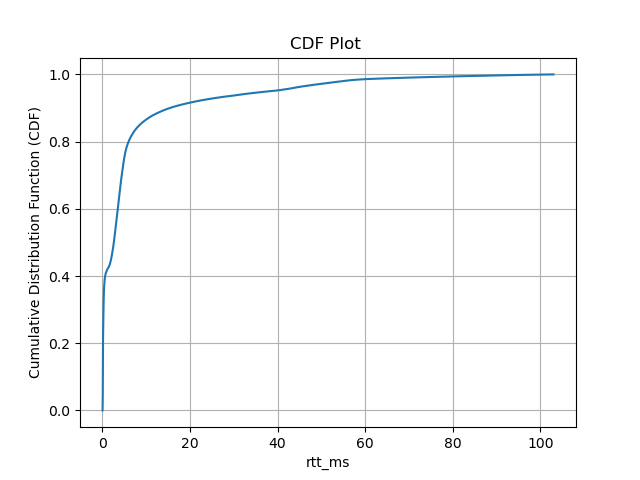
\includegraphics[width=0.75\textwidth]{Figures/rtt_cdf1.png}
    \caption[CDF of RTT in ms]{CDF of RTT in ms}
    \label{fig:rttcdf}
    \bigskip
\end{figure}

%----------------------------------------------------------------------------------------

\section{Packet Loss}

Packet loss is another important metric for detecting congestion events. High packet loss can imply queue buildup and hence, congestion in the network. We calculate packet losses at points both before and after our tapping point in the network. The packet losses occurring after the tapping point i.e. inside the campus network will be seen as a re-transmission event in the downlink pcap trace. The packet losses occurring before the tapping point i.e. on the internet side, can be seen as re-ordering events in the downlink trace. The approach for calculating losses inside the campus is pretty straightforward as we just have to detect retransmission events. We maintain a hash table corresponding to every packet using the flow four-tuple and the packet sequence number and record the time instance when see another packet of the same flow with the same sequence number. For calculating the losses on the internet side, we use a hole-filling-based approach. Algorithm \ref{alg:packet loss} showcases our approach to calculate packet loss on the internet side.

\begin{algorithm}[htpb]
\bigskip
\begin{algorithmic}
\State initialize hash-tables $nextsequencenumber$,$holes$ \Comment{Hash-tables per flow}
\For{$packet$ in $pcap$}
\For{$hole$ in $holes$}
\If{$packet.sequencenumber$ between $hole.start$ and $hole.end$}
    \If{\(packet.ts - hole.ts \geq packet.RTT\)}
        \State record $packet.ts$
        \State increment $internetloss$
    \EndIf
\EndIf 
\EndFor
\If{$nextsequencenumber[flow] \neq packet.nextsequencenumber$} 
    \State $hole.ts \gets packet.ts$
    \State $hole.start \gets nextsequencenumber[flow]$
    \State $hole.end \gets packet.nextsequencenumber$
    \State $holes[flow] \gets hole$
\EndIf

$nextsequencenumber[flow] \gets packet.nextsequencenumber$
\EndFor
\State state $internetloss$
\end{algorithmic}
\caption[Packet Loss]{Packet Loss}
\label{alg:packet loss}
\bigskip
\end{algorithm}

Here, $nextsequencenumber$ and $holes$ are hash tables that store, the next expected sequence number and the different holes encountered for a flow respectively. The key thing in the algorithm is to differentiate between in-network re-ordering and packet loss events. The time between the appearance of the hole and the actual packet is used to differentiate between the two events. Using the RTT estimation algorithm described above, we check if the time difference \( (t_p - t_h) \geq  RTT \), where $t_p$ is the time when the packet actually arrived and $t_h$ is the time when it was expected to arrive. If the condition is satisfied, then it's a packet loss event, otherwise it is an in-network re-ordering event. This is because it will take at least an RTT amount of time for the packet to get re-transmitted if it has been lost. While calculating packet losses, we also need to make sure the packet which we are looking at, is a data packet. We check this by looking at the payload length of a packet. The minimum size of a packet to be transmitted over the Ethernet is 60 bytes(excluding the checksum). The size of an ACK packet is 54 bytes, hence a 6-byte padding is added at the end of an ACK packet. We check if the payload length i.e. \( (packetlen - headerlen - 4) > 6 \), (where 4 bytes is the checksum size) to classify the packet as a data packet and then run the above algorithm on it. We finally report the internet side loss and the campus side loss at the end.

%----------------------------------------------------------------------------------------

\section{Other Key Metrics}

Several other metrics help us in better understanding the characteristics of TCP internet traffic and are useful meta-data for creating new algorithms.

\subsection{Asymmetry}

Detecting asymmetry is an important factor to look into to understand a network. It can happen at times, that a packet flows through a different router in its downlink journey, but takes a different path during its uplink journey. Asymmetry in a network can affect the calculation of metrics such as RTT measurement, as they rely on both the uplink and downlink traffic.

\begin{algorithm}[ttpb]
\bigskip
\begin{algorithmic}
\State initialize hashtable $synpackets$ \Comment{SYN packets for each flow}
\State $asymmetricflows \gets 0$
\For{$packet$ in $uplink$}
    \If{$packet$ is $SYN$}
        \State $synpackets[flow] \gets 1$
    \EndIf
\EndFor
\For{$packet$ in $downlink$}
    \If{$packet$ is $SYN-ACK$}
        \If{$flow$ not in $synpackets$}
            \State increment $asymmetricflows$
        \Else
            \State remove $flow$ from $synpackets$
        \EndIf
    \EndIf
\EndFor
\For{$flow$ in $synpackets$}
    \State increment $asymmetricflows$
\EndFor
\end{algorithmic}
\caption[Asymmetry Detection]{Asymmetry Detection}
\label{alg:asymmetry}
\bigskip
\end{algorithm}

Algorithm \ref{alg:asymmetry} shows how to detect asymmetry in a network. We maintain a hashtable of SYN packets corresponding to each flow and match the packets with the SYN-ACK packets. The number of unmatched packets gives us the amount of asymmetry.

\subsection{Flow Size, Duration and Number of Concurrent Flows}

Flow metrics like flow size, duration, and the number of concurrent flows are important meta-data used in the development of any new algorithm. We calculate the flow sizes by maintaining a hash table with the flow four-tuple as the key and the flow size, both in terms of number of packets and bytes as the value. We increment the flow size, whenever a new packet of the flow is encountered. We calculate the flow duration by maintaining a hash table with the flow four-tuple as the key and a pair of the flow start and end times as the value. The start time is set when we encounter the first packet of the flow. The end-time is updated whenever a new packet of the flow is encountered. We also set a $timeout value$, the time after which, if no more packets of the flow are seen, the flow is considered to end. The flow duration and sizes are reported when the flow ends. Algorithm \ref{alg:concurrent} shows how to calculate the number of concurrent flows at different intervals of time.

\begin{algorithm}[ttpb]
\bigskip
\begin{algorithmic}
\State populate arrays $startTimes,endTimes$ \Comment{pre-processed while calculating flow durations}
\State sort $startTimes,endTimes$
\State $concurrentflows \gets 0$
\State $time \gets stride$
\While{\(time < endTime\)}
\State $num_s \gets $ number of elements in $startTimes$ less than $time$
\State $num_e \gets $ number of elements in $endTimes$ less than $time$
\State $concurrentflows \gets num_s - num_e$
\State record $concurrentflows$
\State increment $time$ by $stride$
\EndWhile
\end{algorithmic}
\caption[Number of Concurrent Flows]{Number of Concurrent Flows}
\label{alg:concurrent}
\bigskip
\end{algorithm}

In the above algorithm, $num_s$ and $num_e$ can be calculated using binary search since the arrays $startTimes$ and $endTimes$ are sorted. The number of concurrent flows at a time is measured by calculating the difference between the number of flows with start time less than $time$ and the number of flows with end time less than $time$. We are basically subtracting the number of flows that have already ended from the number of flows that have started.


% \subsection{Congestion Duration and Inter-arrival time}

% We wrote scripts to analyze congestion duration and inter-arrival time. As we are tapping traffic after the gateway router, we can't see the queue that was formed at the router. We predict congestion by keeping track of N back-to-back packets at line rate where we experimentally determine the correct value of N to be set. We then compute the duration of such congestion events and the time after which the next congestion event occurs for a pcap trace.

%----------------------------------------------------------------------------------------
% Chapter Template

\chapter{Results} % Main chapter title

\label{Chapter4} % Change X to a consecutive number; for referencing this chapter elsewhere, use \ref{ChapterX}

\lhead{Chapter 4. \emph{Results}} % Change X to a consecutive number; this is for the header on each page - perhaps a shortened title

In this section, we present the results obtained and the things we infer upon seeing the measurements. We measure the three key metrics, link utilization, RTT, packet loss along with the asymmetry and flow meta-data as described in the Methodology section and try to correlate them to prove congestion in the network.

\section{Trace collection}
The first strategy for collecting traces was to capture traffic at specific intervals of the day by running our capture tool and then analyzing the captured traffic. We wanted to check for congestion events in the network but this method didn't yield the results that we wanted. Since we were capturing traffic at random intervals, the probability of seeing a congestion event was very low. So we changed our strategy and captured traffic from 9 AM to 9 PM for the whole day on weekdays. The time at which we captured traffic was a recess week in the university, which implied that most of the students were not on campus. Figure \ref{fig:lu} shows the link utilization seen during the recess week during the busy hours,, which hardly touches $8Gbps$ sometimes. Hence, we again got low average link utilization throughout the day. We waited for the recess week to end and the examinations to begin. The traffic captured during the exam week showed high link utilization in general. The link utilization after the recess week is shown in figure \ref{fig:linkutilization}. Since the traffic was captured for 12 hours, the resultant pcap files were very large, accounting to over 500 GB of space on the server and time-consuming to process. So, we dissected the pcap files into smaller files of 10 min duration each using the editcap ~\cite{wireshark} tool from Wireshark.

\begin{figure}[t]
         \centering
         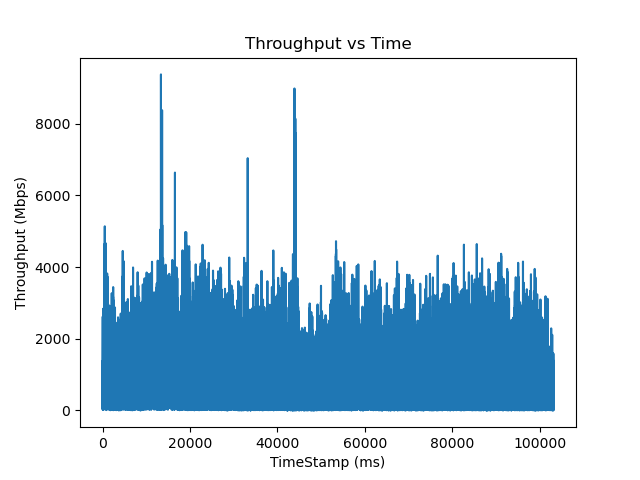
\includegraphics[width=0.6\textwidth]{Figures/link_util_11_29.png}
         \caption[Link utilization between 11:58 AM to 12:08 PM]{Link utilization between 11:58 AM to 12:08 PM}
         \label{fig:lu}
\end{figure}

\section{Link Utilization}
The link speed of the bottleneck link being tapped is $10Gbps$. If we see a saturation at $10Gbps$ for a prolonged period, we can state congestion as one of the possible reasons. We set the window size as 0.4 ms for calculating the throughput as already discussed. During peak hours, we saw saturation events for a prolonged period. Figures \ref{fig:linkutil1} and \ref{fig:linkutil2} show the link utilization during peak hours. The throughput almost constantly touches $10Gbps$ in both the traces. Figures \ref{fig:linkutil3} and \ref{fig:linkutil4} show the link utilization during non-peak hours where the throughput peaks at only some intervals and stays low for the rest of the time. The average link utilization throughout the day as seen from our measurements is around $6Gbps$, with the throughput only peaking during certain hours. Using Ookla's speed test we found out, that the network operators have rate-limited the download speed per machine to $100Mbps$. That means, there must be more than 100 concurrent users requesting data from the servers on the internet to exceed the link capacity of $10Gbps$. It is not expected that 100s of people simultaneously access data from the internet, hence the average link utilization staying low is not a surprising result. However, the link does get saturated around noon, the time when most of the lectures happen and people work in their labs.

\begin{figure}[t]
     \centering
     \begin{subfigure}[h]{0.49\textwidth}
         \centering
         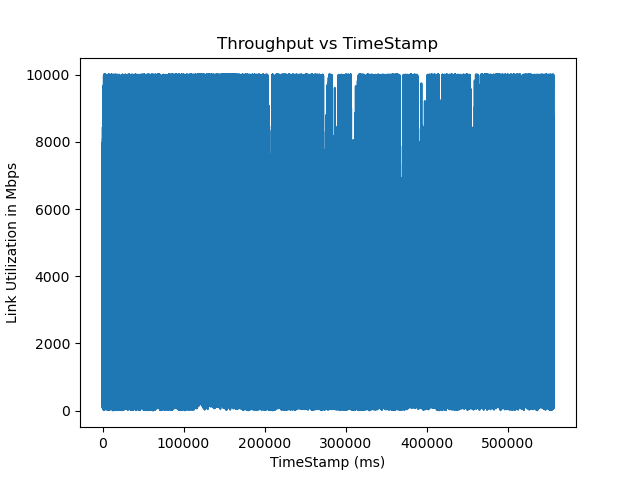
\includegraphics[width=\textwidth]{Figures/saturation_link_1.png}
         \caption[Link Utilization between 11:58 AM to 12:08 PM ]{Link Utilization between 11:58 AM to 12:08 PM}
         \label{fig:linkutil1}
     \end{subfigure}
     \begin{subfigure}[h]{0.49\textwidth}
         \centering
         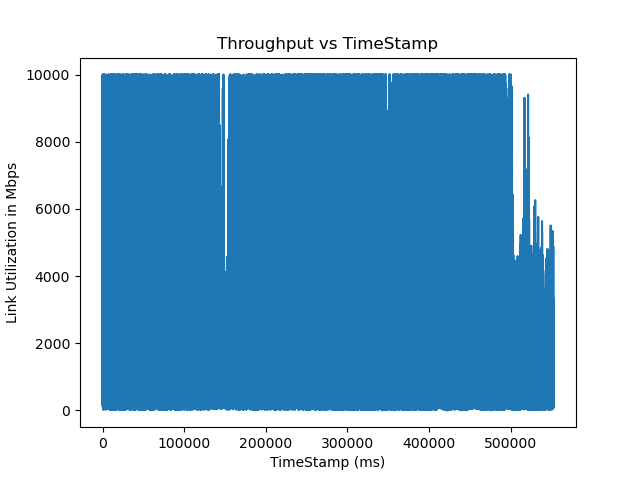
\includegraphics[width=\textwidth]{Figures/saturation_link_2.png}
         \caption[Link Utilization between 12:08 PM to 12:18 PM ]{Link Utilization between 12:08 PM to 12:18 PM }
         \label{fig:linkutil2}
     \end{subfigure}
     \begin{subfigure}[h]{0.49\textwidth}
         \centering
         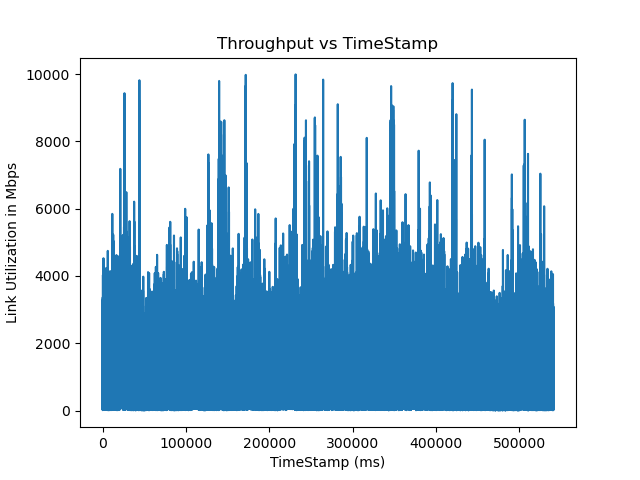
\includegraphics[width=\textwidth]{Figures/saturation_link_3.png}
         \caption[Link Utilization between 10:08 AM to 10:18 AM ]{Link Utilization between 10:08 AM to 10:18 AM }
         \label{fig:linkutil3}
     \end{subfigure}
     \begin{subfigure}[h]{0.49\textwidth}
         \centering
         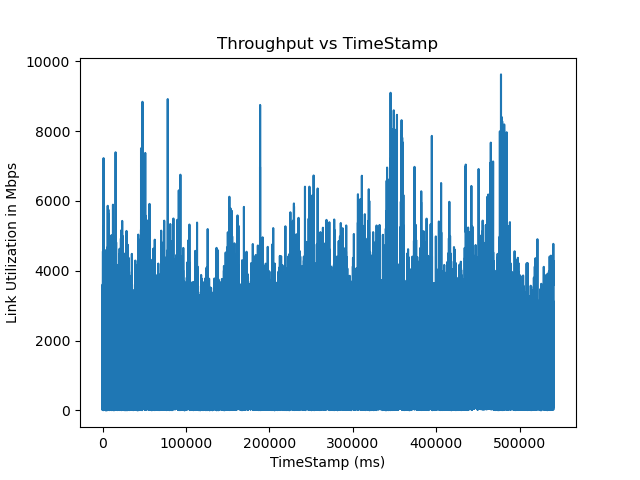
\includegraphics[width=\textwidth]{Figures/saturation_link_4.png}
         \caption[Link Utilization between 10:18 AM to 10:28 AM ]{Link Utilization between 10:18 AM to 10:28 AM }
         \label{fig:linkutil4}
     \end{subfigure}
     \bigskip
     \caption[Link Utilization during peak and non-peak hours]{Link Utilization during peak and non-peak hours}
     \label{fig:linkutilization}
     \bigskip
\end{figure}


%----------------------------------------------------------------------------------------

\section{RTT}
We measure the RTT for the internal leg of a flow using the algorithm discussed previously. The RTT is computed for all flows throughout their lifetime in the pcap trace. Figure \ref{fig:rttcomp} shows the internal leg of the RTTs for two traffic captures. For better understanding and visualizing the CDF, we've plotted the CDF of RTTs up to the 99th percentile. Figure \ref{fig:rtt1} has high RTT values with the 99th percentile recorded at 250ms because of saturation in the traffic capture, while figure \ref{fig:rtt2} has comparatively lower RTT values with the 99th percentile recorded at 102 ms. The RTT values indeed increase by a multiple of 2.5x in figure \ref{fig:rtt1} because of high link utilization, which results in packets getting queued in the buffer and the queueing delay factor being included in the RTT. We also measure the complete leg RTT of the flows using the TCP handshake as discussed previously. Figure \ref{fig:rttcomplete} shows the CDF of the complete-leg RTT values calculated using the TCP handshakes of the flows. These RTT values show a considerable shift in values since the studies done 20 years ago~\cite{tcprtt-imc03}. ~\cite{tcprtt-imc03} states that around 50\% of the RTT samples have RTT lesser than 100ms, whereas our CDF shows that 50\% of the flows have their RTTs lesser than 2ms. The previous studies also reported 90\% of the flows to be having RTT values lesser than 1s, whereas our measurements state that 90\% of the flows have their RTTs lesser than 200ms. These results show that the RTT values have decreased by a huge factor since the last studies done because of several reasons like CDNs and faster links in the backbone of the internet. Our measurements thus contribute to replenishing the old RTT measurements.

\begin{figure}[t]
     \centering
     \begin{subfigure}[h]{0.49\textwidth}
         \centering
         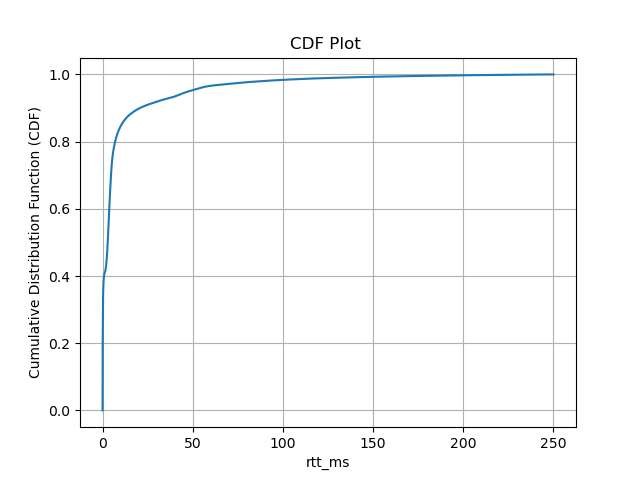
\includegraphics[width=\textwidth]{Figures/rtt_cdf 1.png}
         \caption[CDF of RTT for a saturated traffic capture]{CDF of RTT for a saturated traffic capture}
         \label{fig:rtt1}
     \end{subfigure}
     \begin{subfigure}[h]{0.49\textwidth}
         \centering
         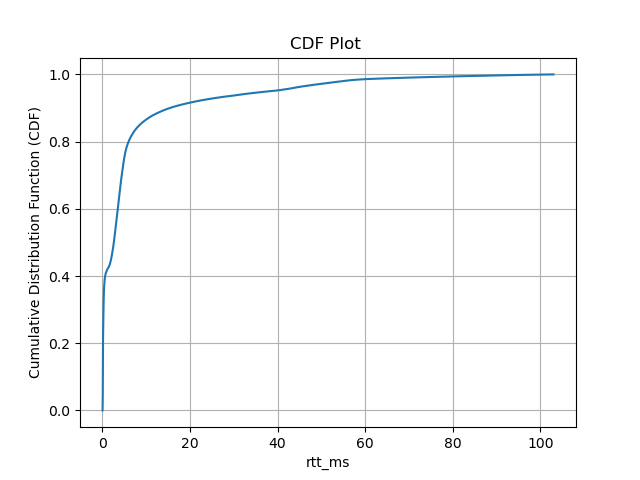
\includegraphics[width=\textwidth]{Figures/rtt_cdf1.png}
         \caption[CDF of RTT for a normal traffic capture]{CDF of RTT for a normal traffic capture}
         \label{fig:rtt2}
     \end{subfigure}
     \caption[Comparison of CDF of RTTs for different traffic captures]{Comparison of CDF of RTTs for different traffic captures}
     \label{fig:rttcomp}
     \bigskip
\end{figure}

\begin{figure}[t]
    \centering
        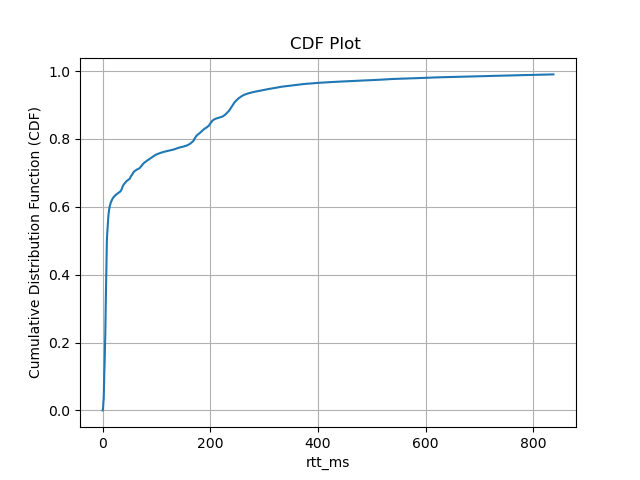
\includegraphics[width=0.6\textwidth]{Figures/complete_rtt.png}
    \caption[CDF of complete leg RTT for a trace]{CDF of complete leg RTT for a trace}
    \label{fig:rttcomplete}
    \bigskip
\end{figure}

%----------------------------------------------------------------------------------------
\section{Packet Loss}

We plot packet losses for a trace by marking the point at which a packet loss happened with a vertical line in Figure~\ref{fig:pktloss}. We mark internet side losses with a red vertical line and the campus(SoC) side losses with a blue vertical line.  One of the possible reasons for packet losses on the campus side being higher in this snapshot might be due to higher losses in the wireless network as compared to the wired network. The average loss rate on the SoC side is seen to be around 0.3\% of the total packets. The packet loss on the internet side for the traces showing high link utilization is lesser than 1\%, somewhere around 0.7\%. The packet losses for the traces showing lower link utilization are higher than 1\% in general. These results make sense because higher packet losses will force flows to decrease their congestion window sizes, which would decrease per-flow throughput leading to lower link utilization. The number of re-ordering events in the network is very large, with around 3-4\% of the total packets getting re-ordered, which compels us to put a check on the time difference between the appearance of the hole in the sequence number chain, and the actual appearance of the packet. The number of packets lost on the internet side may appear to be higher than usual because the time difference currently being considered is kept equal to the RTT of the flow, but some re-ordered packets might arrive later than an RTT because of taking a longer path in the network, but are being counted as packet losses on the internet side. 

\begin{figure}[t]
    \centering
        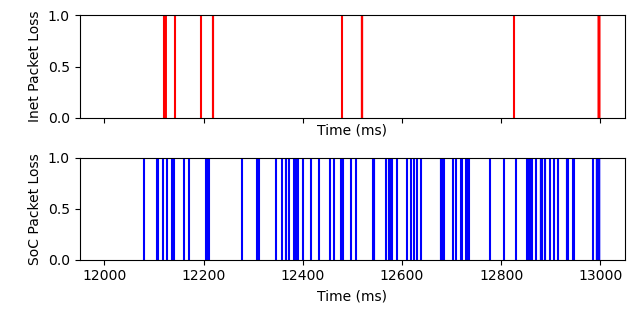
\includegraphics[width=0.75\textwidth]{Figures/packetloss.png}
    \caption[Packet Losses for a trace]{Packet Losses for a trace}
    \label{fig:pktloss}
    \bigskip
\end{figure}

\section{Asymmetry}

We aim to find the number of asymmetric flows in our captures to make sure that our calculations involving both the downlink and uplink pcap files are correct. Let's say a flow $f$ is asymmetric. While calculating the RTT for a capture, we will miss the ACK for some packets of the flow $f$  and it may result in the average RTT being reported wrongly. We find after running our scripts that the number of asymmetric flows is always lesser than 10\% and on average around 7\%. 
Since the number of asymmetric flows is not large, we are able to measure the RTTs of almost all the packets.
%----------------------------------------------------------------------------------------

\section{Other Flow Metrics}

\begin{figure}[t]
    \centering
        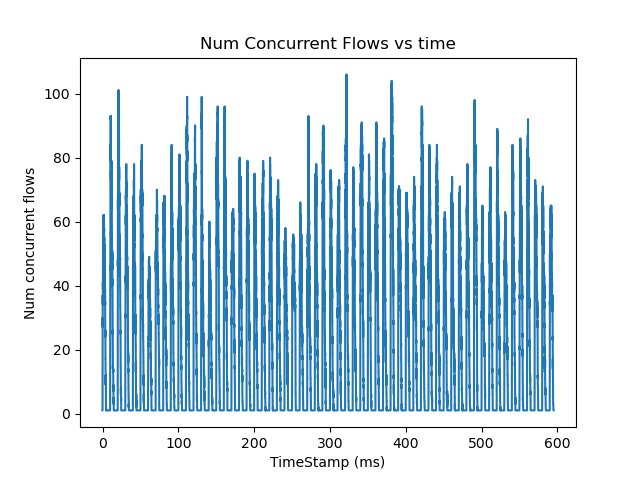
\includegraphics[width=0.75\textwidth]{Figures/concurrent_flows.png}
    \caption[Number of Concurrent Flows]{Number of Concurrent Flows}
    \label{fig:concurr}
    \bigskip
\end{figure}

Figure \ref{fig:concurr} shows the plot of the number of concurrent flows vs time for one of the traffic captures. The number of concurrent flows is an important meta-data used in designing new algorithms. The graph shows that the maximum number of concurrent flows at any point of time is 106. If we are designing a new algorithm for AQM, the metric of the number of concurrent flows will be handy for deciding the number of queues required to accommodate all the flows.

\begin{figure}[t]
    \centering
        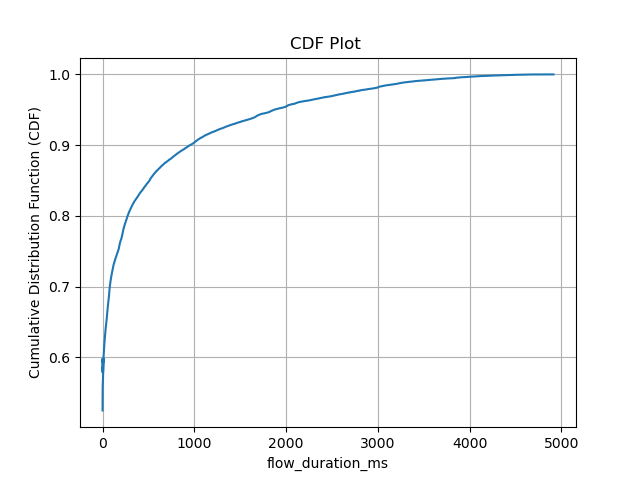
\includegraphics[width=0.75\textwidth]{Figures/flow_duration_cdf.png}
    \caption[Flow duration in ms]{Flow Duration in ms}
    \label{fig:dur}
    \bigskip
\end{figure}

Figure \ref{fig:dur} shows the cdf of the flow duration for the pcap trace. We see from the graph that 60\% of the flows have a duration very close to 0 ms. This tells us that most of the flows are short-lived. Other than that, 90\% of the flows have a duration of less than 1s, and only 10\% of the flows have their  \( duration > 1s \)  with the maximum flow duration being $5s$. Flow duration is another important meta-data that gives us information about the lifetime of a flow, and gives us the proportion of the number of short and long flows in the network which helps us in understanding the network composition better.

\begin{figure}[t]
     \centering
     \begin{subfigure}[h]{0.49\textwidth}
         \centering
         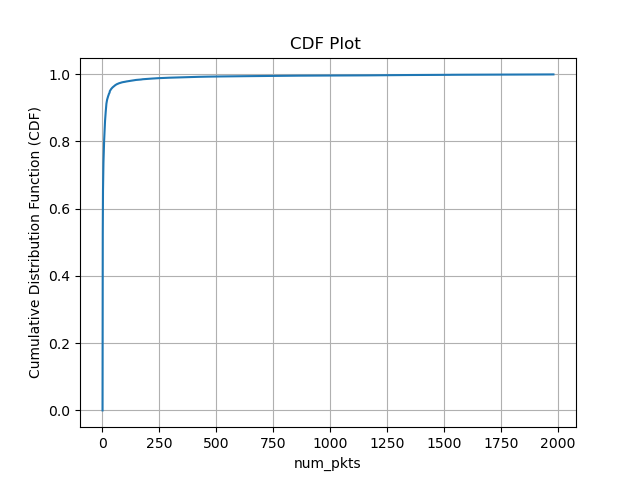
\includegraphics[width=\textwidth]{Figures/num_pkts_cdf.png}
         \caption[CDF of number of packets of flows]{CDF of number of packets of flows}
         \label{fig:pkts1}
     \end{subfigure}
     \begin{subfigure}[h]{0.49\textwidth}
         \centering
         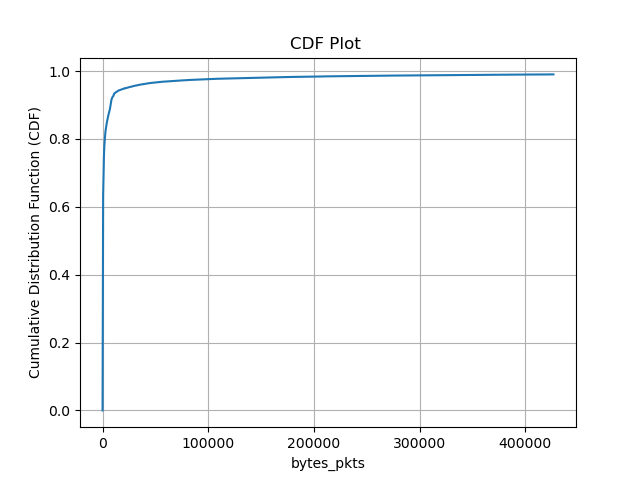
\includegraphics[width=\textwidth]{Figures/byte_pkts_cdf.png}
         \caption[CDF of number of bytes of flows]{CDF of number of bytes of flows}
         \label{fig:pkts2}
     \end{subfigure}
     \caption[Flow sizes]{Flow sizes}
     \label{fig:pktcdf}
     \bigskip
\end{figure}

Figure \ref{fig:pktcdf} shows the cdf of the number of packets of flows \ref{fig:pkts1} and the number of bytes of flows \ref{fig:pkts2}. As seen from figure \ref{fig:dur} of the flow durations, most of the flows are short lived. Hence, it is imperative that sizes of most of the flows will be small. The CDFs show that around 90\% of the flows have number of packets smaller than 250 and he number of bytes smaller than 7500 bytes. Hence, from these graphs we get to know that most of the flows in the network are short-lived with small flow sizes.



%----------------------------------------------------------------------------------------

\section{Correlation between Link Utilization,Packet Loss and RTT}

We consider a pcap trace which has both regions of high link utilization and low link utilization to show congested regions. Figure \ref{fig:linkutil_satur} shows the pcap trace being considered for the correlation. The pcap trace experiences a high jump in link utilization around the 400s mark. If we see a correspondence between the RTT, link utilization and packet losses around this point, we'll be able to pinpoint a congestion event.

We want to consider a flow, which exists in both regions of low link utilization and high link utilization and see how different metrics of the flow change when it goes through this transition. Figure \ref{fig:corr} shows the correlation between the RTT values of one of such flows and the link utilization. \ref{fig:corr} shows that the RTT values of the flow experience a spike as soon as the link utilization starts touching $10Gbps$ and the RTT increases in general through the high link utilization region.Since we are monitoring the internal leg RTT, the graph suggests that there is congestion inside the campus network as the RTT values of the internal leg are increasing.

Figure \ref{fig:correlation} further shows the packet losses along with the RTT and link utilization. As the link utilization increases, the RTT values of a flow being monitored increase continuously and a cluster of packet losses on the internet side is also seen. This graph, on the contrary, suggests that congestion is happening on the internet side due to an increase in packet losses on the internet side. The packet losses happen due to buffer overflow in a congested link before the campus. 

These results show the occurrence of congestion, but locating the point of congestion requires further study.

\begin{figure}[t]
    \centering
        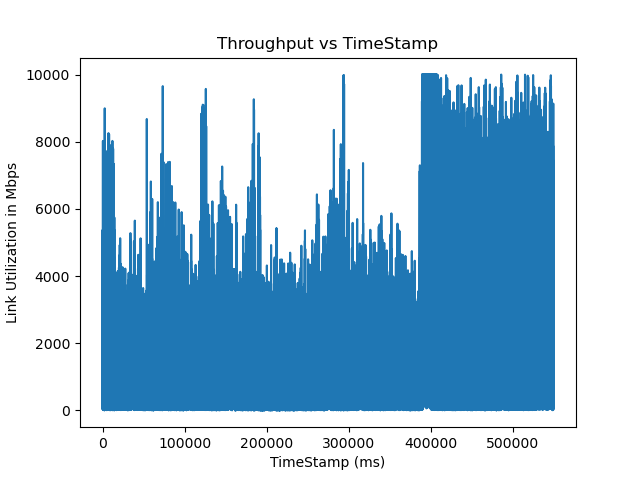
\includegraphics[width=0.75\textwidth]{Figures/link_util_satur.png}
    \caption[Link Utilization of the trace being considered]{Link Utilization of the trace being considered}
    \label{fig:linkutil_satur}
    \bigskip
\end{figure}

\begin{figure}[t]
    \centering
        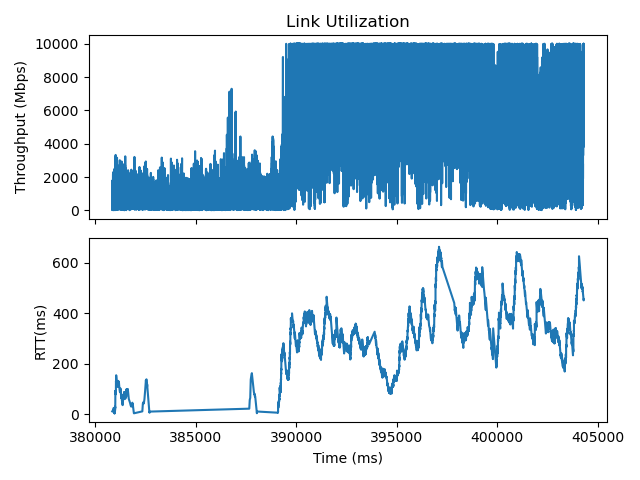
\includegraphics[width=0.75\textwidth]{Figures/RTT_saturation.png}
    \caption[Correlation between RTT of a flow and link utilization]{Correlation between RTT of a flow and link utilization}
    \label{fig:corr}
    \bigskip
\end{figure}

\begin{figure}[t]
    \centering
        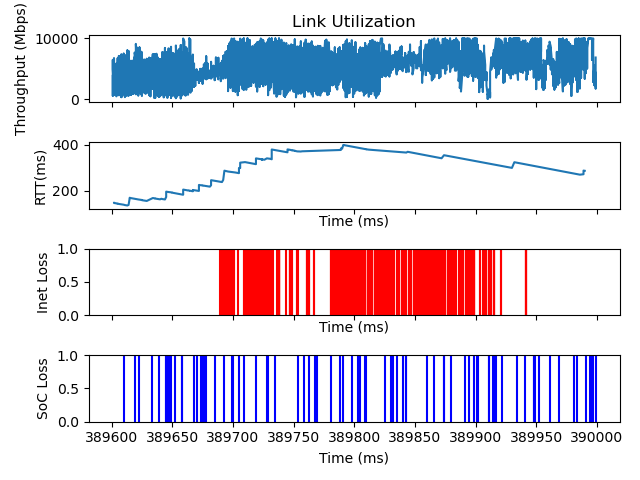
\includegraphics[width=0.75\textwidth]{Figures/correlation.png}
    \caption[Correlation between RTT,link utilization and packet loss]{Correlation between RTT,link utilization and packet loss}
    \label{fig:correlation}
    \bigskip
\end{figure}

%----------------------------------------------------------------------------------------
% Chapter Template

\chapter{Conclusion} % Main chapter title

\label{Chapter 5} % Change X to a consecutive number; for referencing this chapter elsewhere, use \ref{ChapterX}

\lhead{Chapter 5. \emph{Conclusion}} % Change X to a consecutive number; this is for the header on each page - perhaps a shortened title

%----------------------------------------------------------------------------------------

%\section{Summary}

% future. not just one measurement after an other
% desigining the systems that can run on programmable switches. deployable across different vantage points. and do differential analysis and verifiability.

% packet brokering. it is one idea in the overall genenral system design that could enable this kind of continuous real time monitoring and metric collecting sytem in the dataplane.

We have built and deployed a system that is able to monitor live traffic at the network edge, that can handle traffic from multiple 10 Gb/s links. The system can perform anonymization of the traffic at line rate using a P4 programmable switch. Using our system for packet capture, we measured important metrics in the network such as link utilization, packet loss, RTT, asymmetry and other flow meta-data. These measurements can  help us better understand modern network characteristics. We correlate three of the metrics i.e. link utilization, packet losses and RTT to infer congestion events in the network. These measurements also help us in designing new algorithms for the future.

%----------------------------------------------------------------------------------------

\section{Future Work}

\subsection{Extend measurements to the data plane}

We can extend our methodology to directly make measurements in the data plane itself using a P4 program. Our current methodology involves offline analysis of captured data on our server. Taking measurements on the switch itself will provide us with real-time metrics and will be helpful for us in timely identifying any problems with the network. For example, we can immediately notify the network operators if we see considerable losses in the network and provide them data to better troubleshoot the problem.

\subsection{Pinpoint the location of congestion events}

We current have evidence that there are congestion events at the edge. What we have not yet been able to do is to pinpoint the location of the congestion event. Locating the place of congestion requires further in-depth analysis of different metrics.

\subsection{Further categorize internet side losses}

We can further try to classify internet-side losses. The losses can either happen due to link corruption or link congestion. Packet loss due to link corruption is a major problem in large warehouse-scale data centers. Hence categorizing the internet side losses will provide us with new insights into the kind of losses happening on the internet.
%----------------------------------------------------------------------------------------
\input{Chapters/Chapter6}
%\input{Chapters/Chapter7}

%-------------------------------------------------------------------------------
%	THESIS CONTENT - APPENDICES
%-------------------------------------------------------------------------------

\addtocontents{toc}{\vspace{2em}} % Add a gap in the Contents, for aesthetics

\appendix % Cue to tell LaTeX that the following 'chapters' are Appendices

% Include the appendices of the thesis as separate files from the Appendices
% folder
% Uncomment the lines as you write the Appendices

\input{Appendices/AppendixA}
%\input{Appendices/AppendixB}
%\input{Appendices/AppendixC}

\addtocontents{toc}{\vspace{2em}} % Add a gap in the Contents, for aesthetics

\backmatter

%-------------------------------------------------------------------------------
%	BIBLIOGRAPHY
%-------------------------------------------------------------------------------

\label{Bibliography}

\lhead{\emph{Bibliography}} % Change the page header to say "Bibliography"

\printbibliography

\end{document}
